\Chapter{Experimentos}{Trabajo y Resultados}

\section{Conjuntos de datos}
\index{Conjuntos de datos}

Los diferentes conjuntos de datos utilizados para medir el rendimiento
de las distintas implementaciones han sido obtenidos de
\href{http://jobshop.jjvh.nl/}{(HTTP) Jobshop Instances}
o diseñados a mano.

Para desarrollar el programa se han utilizado conjuntos de datos
personalizados hechos a mano para facilitar la creación
de pruebas de software que comprueben el correcto funcionamiento
del algoritmo.

Para ejecutar las pruebas se han utilizado porciones de conjuntos
de datos obtenidos de \href{http://jobshop.jjvh.nl/}{(HTTP) Jobshop Instances}.
En particular se ha utilizado el $50\percentsign$ del conjunto
`abz5' (5x5) o el $100\percentsign$ de `ft06' (6x6).

\begin{notebox}
    \index{Tamaño del problema}
    Un conjunto de datos tiene un tamaño de $A$x$B$ cuando
    está compuesto por $A$ trabajos y $B$ tareas.
\end{notebox}

\pagebreak

\section{Equipos de Prueba}
\index{Equipos de Prueba}

\subsection{Arquitectura x86}
\index{Equipos de Prueba!Arquitectura x86}

Se han utilizado 3 equipos diferentes para tomar y contrastar las mediciones.

\subsubsection{OS}
\index{Equipos de Prueba!Arquitectura x86!OS}

\begin{center}
    \begin{table}[h]
        \centering
        \begin{tabular}{ l | l l l }
            \hline
            ID & Tipo & OS & Versión \\
            \hline
            0 & Escritorio & Arch Linux & 6.9.6-arch1-1 \\
            1 & Servidor & Debian Linux 12 \italic{`Bookworm'} & 6.1.0-16-amd64 \\
            2 & Portátil & Debian Linux 12 \italic{`Bookworm'} & 6.1.0-16-amd64 \\
            \hline
        \end{tabular}
        \caption{Equipos de prueba, arquitectura x86: OS}
    \end{table}
\end{center}

\subsubsection{CPU}
\index{Equipos de Prueba!Arquitectura x86!CPU}

\begin{center}
    \begin{table}[h]
        \centering
        \begin{tabular}{ l | l l l l }
            \hline
            ID & Familia & Modelo & Hilos & Reloj \\
            \hline
            0 & Intel & Core I7-9700F & 8c8t & 4.7GHz \\
            1 & Intel & Xeon-E5450 & 4c4t & 3GHz \\
            2 & AMD & Ryzen 7 5700U & 8c16t & 4.3GHz \\
            \hline
        \end{tabular}
        \caption{Equipos de prueba, arquitectura x86: CPU}
    \end{table}
\end{center}

\subsubsection{RAM}
\index{Equipos de Prueba!Arquitectura x86!RAM}

\begin{center}
    \begin{table}[h]
        \centering
        \begin{tabular}{ l | l l r r}
            \hline
            ID & RAM & Formato & Tipo & Reloj \\
            \hline
            0 & 64GB & 4x16 & DDR4 & 3200MHz \\
            1 & 8GB & 2x4 & DDR3 & 2666MHz \\
            2 & 16GB & 2x8 & DDR4 & 3200MHz \\
            \hline
        \end{tabular}
        \caption{Equipos de prueba, arquitectura x86: RAM}
    \end{table}
\end{center}

\pagebreak

\section{Método de medición}

Todas las versiones imprimen por salida estándar datos que posteriormente son
procesados en formato CSV:

\begin{itemize}[itemsep=0.25px]
    \item Lenguaje
    \item Número de hilos
    \item Porcentaje del trabajo resuelto
    \item Trabajos
    \item Tareas
    \item Trabajadores
    \item Tiempo de ejecución
    \item Planificación
    \item \italic{Makespan}
\end{itemize}

La alta complejidad del JSP implica que un mínimo aumento en el tamaño del problema
puede implicar que el algoritmo no finalice su ejecución en un tiempo polinomial.
Por ello, en lugar de tomar una única medición al inicio y final de la ejecución
se ha optado por utilizar un objeto personalizado que toma mediciones en intervalos
predefinidos\footnote{Véase \ref{lst:Chronometer}}.
De esta forma, de una única ejecución se podría obtener:

\begin{itemize}[itemsep=0.25px]
    \item Tiempo de inicio.
    \item Tiempo necesario para resolver el $10\percentsign$ del problema.
    \item Tiempo necesario para resolver el $20\percentsign$ del problema.
    \item \dots
    \item Tiempo necesario para resolver el $90\percentsign$ del problema.
    \item Tiempo necesario para resolver el $100\percentsign$ del problema.
\end{itemize}

\section{Métricas}

A continuación se listan las diferentes métricas observadas a la hora
de estudiar y criticar las implementaciones del algoritmo:
\begin{itemize}[itemsep=0.25px]
    \item Tiempo de ejecución - Menor implica mejor.
    \item \italic{Speedup} - Mayor implica mejor.
    \item \italic{Makespan} - Menor implica mejor.
    \item Consumo de CPU \footnote{
        Dependiendo de otras métricas, el consumo de CPU se
        puede utilizar para `desempatar' algoritmos que
        aparentemente tengan los mismos resultados,
        en cuyo caso menor implica mejor.
    }.
\end{itemize}

\subsection{\italic{Speedup}}
\index{Speedup}

Sean $T_1$ y $T_0$ dos métricas del tiempo de ejecución
de dos algoritmos distintos ($A0$ y $A1$),
el \italic{speedup} del algoritmo $A0$ respecto al $A1$ ($S_{A0,A1}$) es:
$$
    S_{A0,A1} = T_1 / T_0
$$

\begin{examplebox}
    Si el algoritmo $A0$ tardó $5s$ en finalizar y
    $A1$ tardó $10s$, el \italic{speedup} ($S_{A0,A1}$):
    $$
        S_{A0,A1} = T_1 / T_0 = 10 / 5 = 2
    $$
    $A0$ es el doble de rápido que $A1$.
\end{examplebox}

Por lo tanto:
$$ S_{A0,A1} = 1 \rightarrow T_1 = T_0 $$ 
$$ S_{A0,A1} > 1 \rightarrow T_1 > T_0 $$ 
$$ S_{A0,A1} < 1 \rightarrow T_1 < T_0 $$

\subsection{\italic{Makespan}}
\index{Makespan}

El \italic{makespan} es el tiempo necesario para completar
todos los trabajos de un conjunto de datos,
es el `resultado' que genera el algoritmo.

Lógicamente, existe un \italic{makespan} óptimo para cada
conjunto de datos, el mínimo.
No obstante, el algoritmo desarrollado en este proyecto
no tiene la certeza de obtener ese resultado siempre.
Por ello, si una implementación $A$ retorna
resultados con un \italic{makespan} que otra $B$,
$A$ es mejor que $B$ \footnote{
    Suponiendo que el resto de métricas entre $A$ y $B$
    son lo suficientemente similares.
}.

\section{Resultados y Análisis}
\index{Resultados}

\subsection{Complejidad del problema}
\index{Resultados!Complejidad del problema}


En la siguiente gráfica (figura \ref{fig:Runtime_One_Problem_Linear}),
se puede ver el tiempo de ejecución
necesario para completar el problema utilizando uno de los
algoritmos.

\begin{figure}[h]
    \centering
    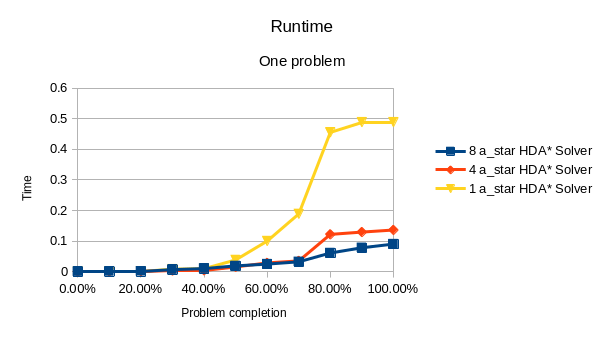
\includegraphics[width=\textwidth]{Media/Ch2/Runtime_One_Problem_Linear.png}
    \caption{Tiempo de ejecución de un único problema.}
    \label{fig:Runtime_One_Problem_Linear}
\end{figure}

Como se puede ver, el diagrama es de poca utilidad debido a la
complejidad del problema.
Para poder observar con mejor los resultados,
se utiliza un eje vertical con una escala logarítmica
(figura \ref{fig:Runtime_One_Problem_Log}).

\begin{figure}[h]
    \centering
    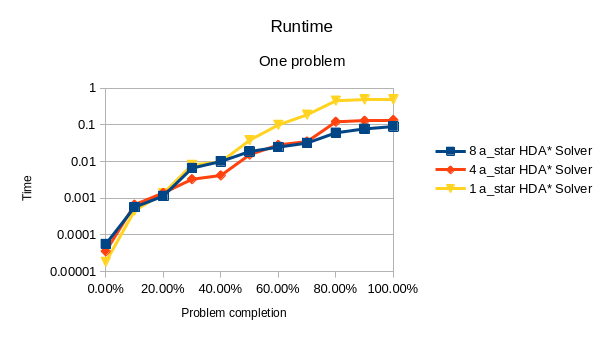
\includegraphics[width=\textwidth]{Media/Ch2/Runtime_One_Problem_Log.png}
    \caption{Tiempo de ejecución de un único problema (escala logarítmica).}
    \label{fig:Runtime_One_Problem_Log}
\end{figure}

Estas observaciones verifican que la complejidad del problema
a resolver es cuadrática, como era de esperar.

\begin{notebox}
    Esta sección contiene diversas gráficas de las métricas obtenidas,
    obsérvese con detalle la escala utilizada en el eje de ordenadas de cada una
    ya que en algunos casos será logarítmica.
\end{notebox}

\subsection{Comparativa de heurísticos}
\index{Resultados!Heurísticos}

Como ya se discutió en la sección sobre optimización (\ref{ssec:Heuristicos}),
existen varias implementaciones de la función heurística que da al algoritmo
A* su particular comportamiento de ir `dirigido' hacia la solución.
En esta investigación se han implementado dos heurísticos:
uno de ellos busca una solución que se acerque a la óptima lo máximo posible
mientras que el otro busca la solución priorizando la velocidad del algoritmo.
A continuación se comparan los heurísticos utilizando la implementación paralela HDA*.

En primer lugar se observa que existe un limitado número de soluciones
propuestas, las más comunes siendo también las más bajas: 452 y 472.
Respecto al tiempo de ejecución, las pruebas que utilizan el heurístico rápido
reducen el tiempo de ejecución en varias magnitudes.

\begin{figure}[h]
    \begin{subfigure}{.5\textwidth}
        \begin{center}
            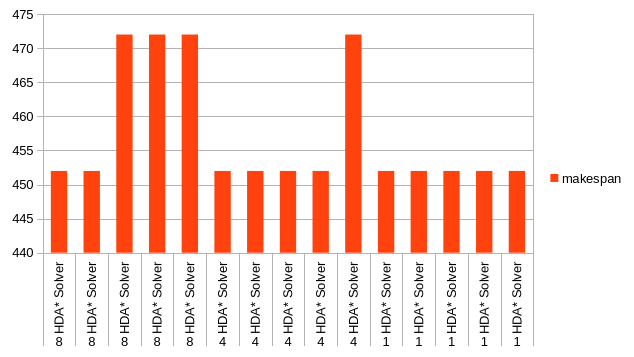
\includegraphics[width=\textwidth]{Media/Ch2/Makespan_Slow_HDA.png}
            \subcaption{\italic{Makespan} del heurístico lento.}
        \end{center}
    \end{subfigure}
    \begin{subfigure}{.5\textwidth}
        \begin{center}
            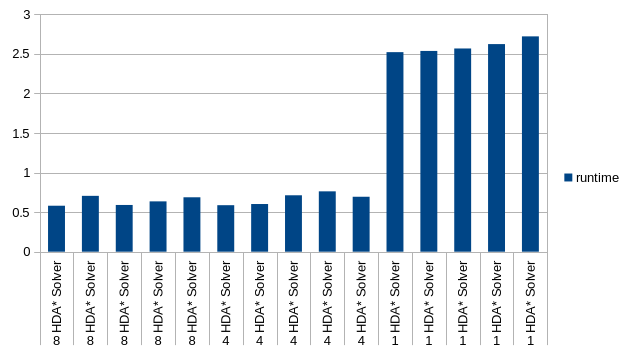
\includegraphics[width=\textwidth]{Media/Ch2/Runtime_Slow_HDA.png}
            \subcaption{Tiempo de ejecución del heurístico lento.}
        \end{center}
    \end{subfigure}
    \caption{Métricas heurístico lento.}
    \label{fig:HeuristicoLento}
\end{figure}

\begin{figure}[h]
    \begin{subfigure}{.5\textwidth}
        \begin{center}
            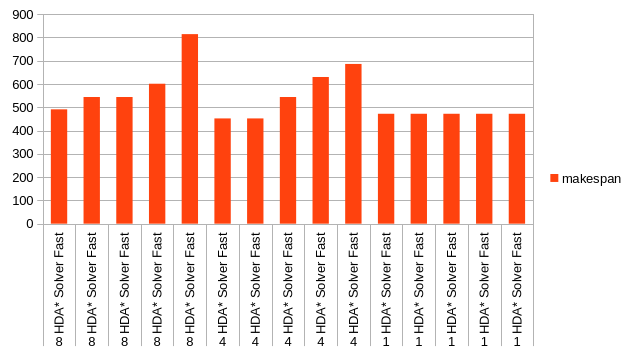
\includegraphics[width=\textwidth]{Media/Ch2/Makespan_Fast_HDA.png}
            \subcaption{\italic{Makespan} del heurístico rápido.}
        \end{center}
    \end{subfigure}
    \begin{subfigure}{.5\textwidth}
        \begin{center}
            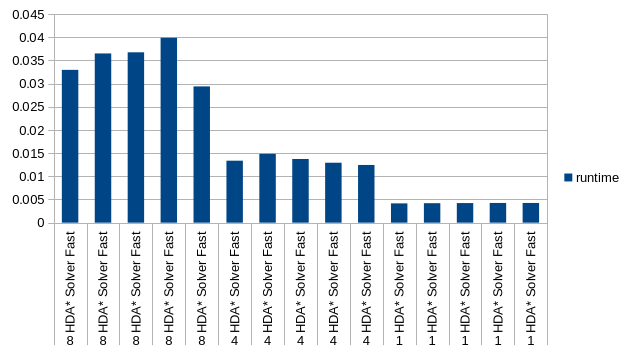
\includegraphics[width=\textwidth]{Media/Ch2/Runtime_Fast_HDA.png}
            \subcaption{Tiempo de ejecución del heurístico rápido.}
        \end{center}
    \end{subfigure}
    \caption{Métricas heurístico rápido.}
    \label{fig:HeuristicoRapido}
\end{figure}

Analizandolas por separado, las ejecuciones que utilizan el heurístico lento
retornaron siempre 452 o 472, los dos mejores resultados y se vieron
beneficiadas por el uso de varios hilos.
Por otro lado, las ejecuciones que utilizan el heurístico rápido
sólo retornaron 452 o 472 en algunas instancias y no se vieron
beneficiadas por el uso de varios hilos
(Véase figuras \ref{fig:HeuristicoLento} y \ref{fig:HeuristicoRapido}).

Sería razonable suponer que el heurístico rápido
sí se vería beneficiado por el paralelismo si el tamaño del
problema fuese lo suficientemente grande.
Para comprobar esta hipótesis, se ha creado un conjunto
con un tamaño mucho mayor (70x10) y se ha obtenido el \italic{speedup}.

\begin{figure}[h]
    \centering
    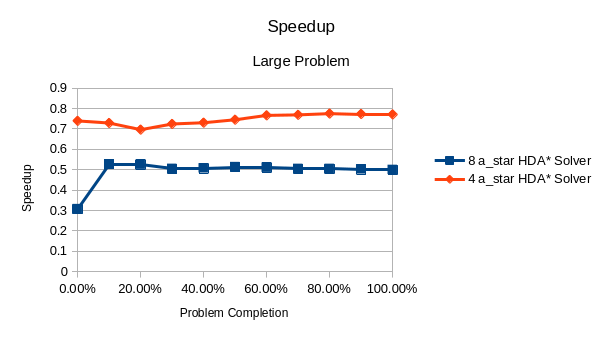
\includegraphics[width=\textwidth]{Media/Ch2/Speedup_Large_Problem.png}
    \caption{\italic{Speedup} en un problema de gran tamaño.}
    \label{fig:Speedup_Large_Problem}
\end{figure}

La gráfica (\ref{fig:Speedup_Large_Problem}) muestra que incluso en un problema de mayor tamaño
la versión monohilo es más rápida que las multihilo.
Esta investigación no ha podido encontrar un conjunto de datos
en el que utilizando el heurístico rápido valga la pena el paralelismo.
No obstante, se ha observado que a medida que el tamaño
del problema incrementa, el \italic{speedup} también se ve incrementando
por lo que si se supone que la tendencia del \italic{speedup}
se mantiene, sería razonable suponer que existe un tamaño de
problema donde sí vale la pena utilizar varios hilos y 
el heurístico rápido.

\subsection{Cuellos de botella en secciones críticas}
\index{Resultados!Cuellos de botella}

Los algoritmos que utilizan estructuras de datos compartidas
para almacenar los nodos y sus costes se ven gravemente
afectadas cuando el tamaño de estas estructuras incrementa.
Como esta información es compartida por todos los hilos,
es necesario acceder a ella de forma serializada,
reduciendo notablemente el \italic{speedup}.

En algunos casos extremos es posible incluso
que versiones monohilo del mismo algoritmo
tengan mejor rendimiento que versiones paralelas.
Nótese que el \italic{speedup} del algoritmo FCFS
cuando se utilizan varios hilos (respecto a un hilo solo)
es inferior a $1$.
(Véase figura \ref{fig:ParalelismoFCFS}).

\begin{figure}[h]
    \begin{subfigure}{.5\textwidth}
        \begin{center}
            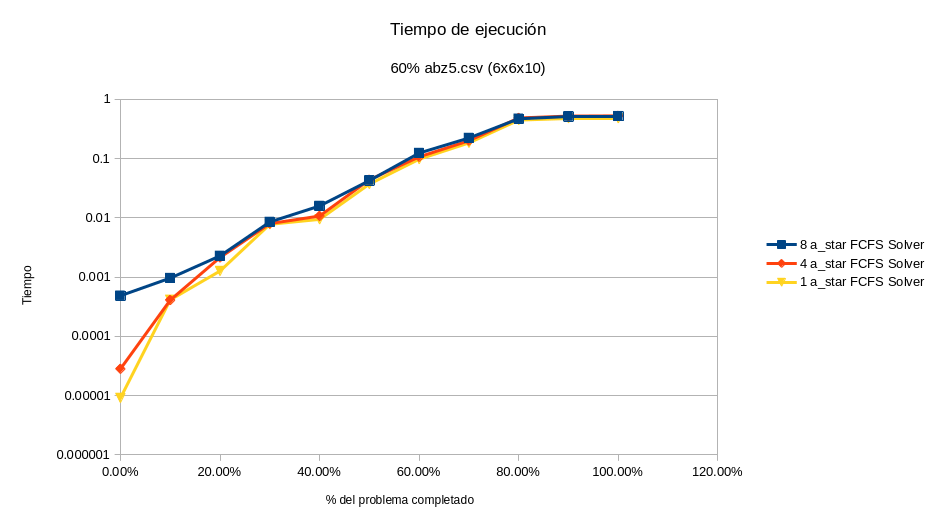
\includegraphics[width=\textwidth]{Media/Ch2/Runtime_FCFS_Log.png}
            \subcaption{Tiempo de ejecución de FCFS.}
        \end{center}
    \end{subfigure}
    \begin{subfigure}{.5\textwidth}
        \begin{center}
            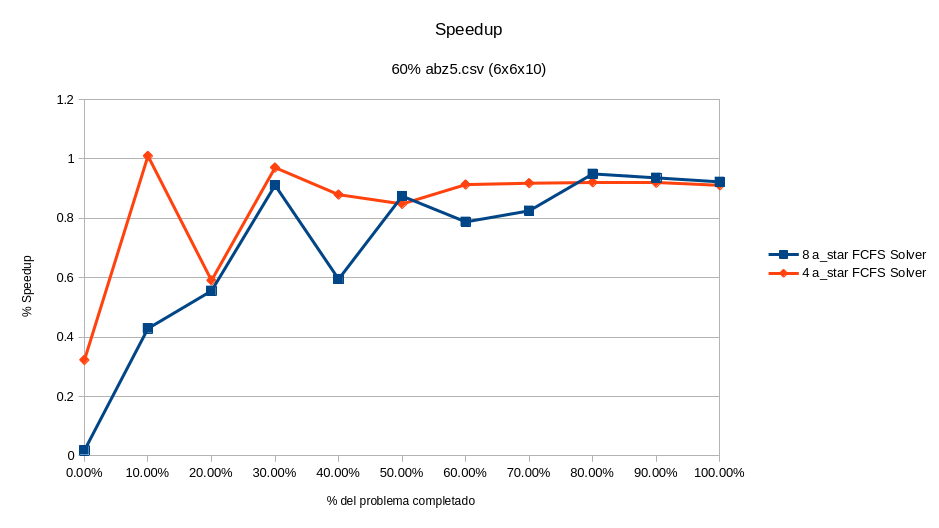
\includegraphics[width=\textwidth]{Media/Ch2/Speedup_FCFS.png}
            \subcaption{\italic{Speedup} de FCFS.}
        \end{center}
    \end{subfigure}
    \caption{Métricas de paralelismo en FCFS.}
    \label{fig:ParalelismoFCFS}
\end{figure}

Por otro lado, algoritmos como el HDA*
que utilizan una estructura de datos privada para cada hilo
no ven sus tareas serializadas,
incrementando notablemente el \italic{speedup}
(Véase figura \ref{fig:ParalelismoHDA}).

\begin{figure}[h]
    \begin{center}
        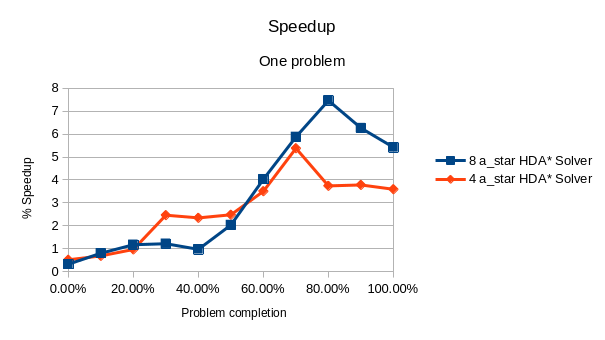
\includegraphics[width=\textwidth]{Media/Ch2/Speedup_One_Problem.png}
    \end{center}
    \caption{\italic{Speedup} de HDA*.}
    \label{fig:ParalelismoHDA}
\end{figure}

Nótese que al inicio del problema (aproximadamente hasta completar el $30\percentsign$)
la versión monohilo de los algoritmos es más rápida que cualquier multihilo.
Esto se debe a que para tamaños de problema muy pequeños
el coste de crear $N$ hilos es superior al de resolver el problema
utilizando uno sólo.

Si se observa el \italic{speedup} al final del problema,
la versión con cuatro hilos tiene un \italic{speedup}
de $3.5$ mientras que la de ocho tiene $5.5$.
Esto implica que al utilizar cuatro hilos,
el algoritmo ha sido capaz de aprovecharlos casi al máximo
ya que el tiempo de ejecución casi se reduce en 4
veces.
Mientras tanto, al utilizar 8 hilos el algoritmo
no ha sido capaz de rentabilizarlos en la misma proporción.
Este déficit podría deberse a que el tamaño del problema
es demasiado pequeño para aprovechar la cantidad de hilos
o podría deberse al propio diseño del algoritmo.

\subsection{Comparativa de algoritmos}
\index{Resultados!Comparativa de algoritmos}

Como es de esperar, el rendimiento monohilo de todas
las implementaciones es el mismo.
Todas las implementaciones están diseñadas de forma
que al ser ejecutadas con un sólo hilo
el algoritmo sea el A* básico.

\begin{figure}[h]
    \begin{center}
        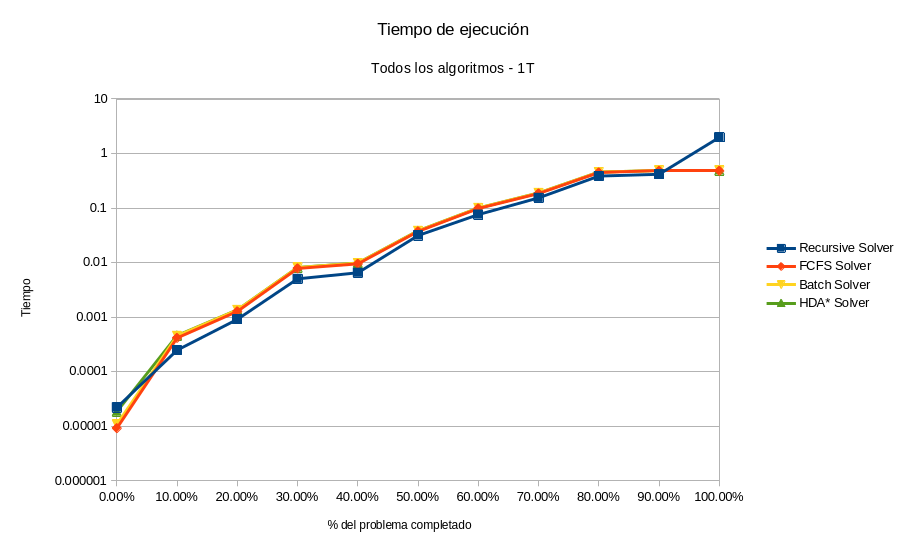
\includegraphics[width=\textwidth]{Media/Ch2/Runtime_All_Algorithms_1.png}
    \end{center}
    \caption{Tiempo de ejecución de todos los algoritmos (1 hilo).}
    \label{fig:MetricasSinglethread}
\end{figure}

\begin{figure}[h]
    \begin{subfigure}{.5\textwidth}
        \begin{center}
            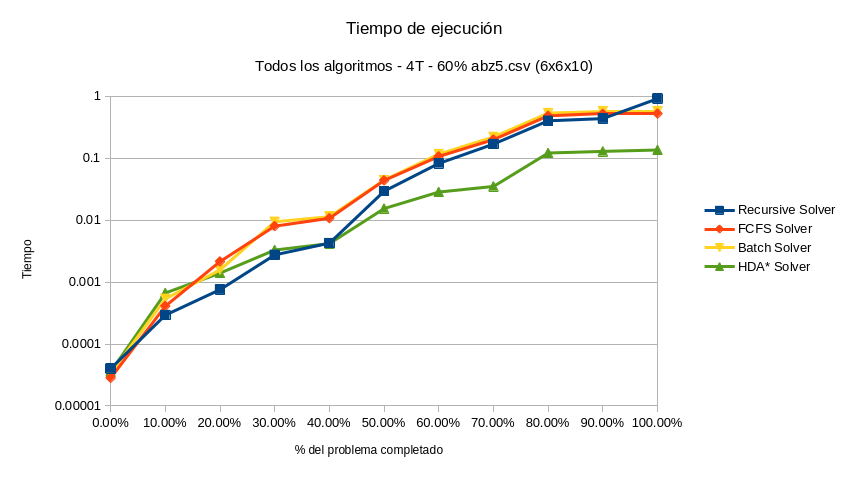
\includegraphics[width=\textwidth]{Media/Ch2/Runtime_All_Algorithms_4.png}
            \subcaption{Tiempo de ejecución de todos los algoritmos (4 hilos).}
        \end{center}
    \end{subfigure}
    \begin{subfigure}{.5\textwidth}
        \begin{center}
            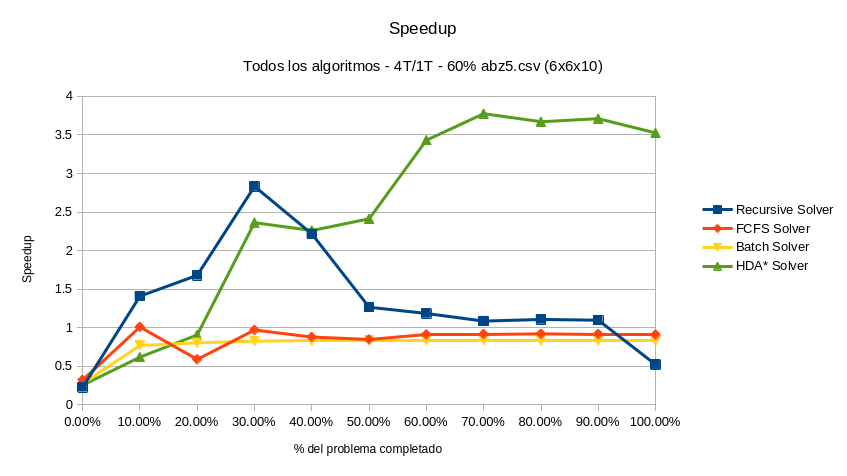
\includegraphics[width=\textwidth]{Media/Ch2/Speedup_All_Algorithms_4.png}
            \subcaption{\italic{Speedup} de todos los algoritmos (4 hilos).}
        \end{center}
    \end{subfigure}
    \caption{Métricas con 4 hilos.}
    \label{fig:Metricas4Thread}
\end{figure}

Al utilizar cuatro hilos (figura \ref{fig:Metricas4Thread}), se puede comenzar a ver una diferencia clara
en el rendimiento del algoritmo HDA*, que obtiene un \italic{speedup}
de casi 4.

\begin{figure}[h]
    \begin{subfigure}{.5\textwidth}
        \begin{center}
            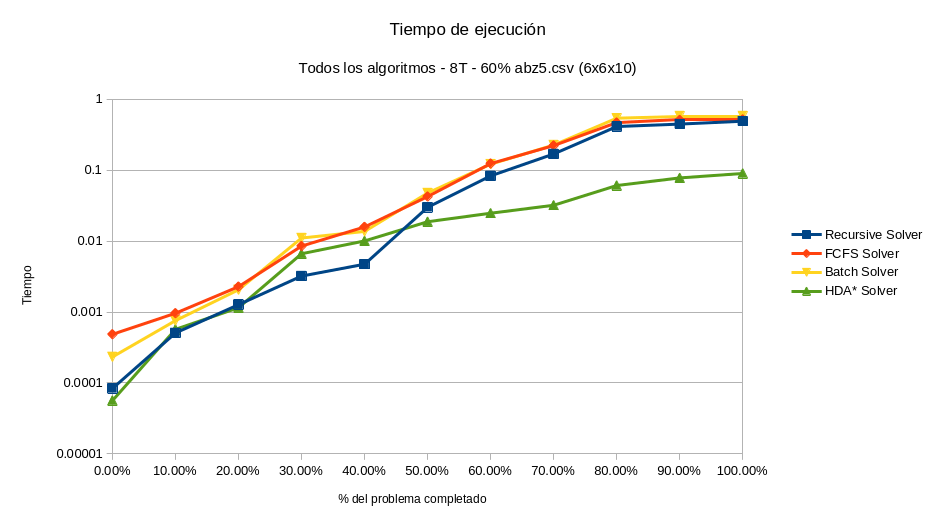
\includegraphics[width=\textwidth]{Media/Ch2/Runtime_All_Algorithms_8.png}
            \subcaption{Tiempo de ejecución de todos los algoritmos (8 hilos).}
        \end{center}
    \end{subfigure}
    \begin{subfigure}{.5\textwidth}
        \begin{center}
            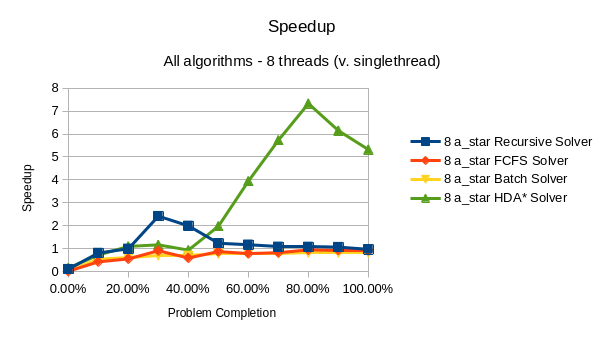
\includegraphics[width=\textwidth]{Media/Ch2/Speedup_All_Algorithms_8.png}
            \subcaption{\italic{Speedup} de todos los algoritmos (8 hilos).}
        \end{center}
    \end{subfigure}
    \caption{Métricas con 8 hilos.}
    \label{fig:Metricas8Thread}
\end{figure}

Al utilizar ocho hilos (figura \ref{fig:Metricas8Thread}), el algoritmo HDA* incremente aún más su diferencia
en el tiempo de ejecución con respecto al resto de algoritmos,
aunque esta vez el \italic{speedup} fluctua más.
De cualquier forma, parece ser capaz de alcanzar casi 8.

La principal conclusión de estas observaciones es que
(al menos en los conjuntos de datos observados)
el paralelismo es sólo rentable si se implementa el HDA*.
En el resto de casos, el paralelismo sólo sirve para
gastar núcleos y ciclos de CPU a cambio de nada.

\pagebreak

\subsection{Casos particulares}
\index{Resultados!Casos particulares}

Vistos los resultados anteriores
se podrían dar como obsoletas algunas de las versiones
paralelas por ofrecer muy pocas mejoras frente a otras
versiones monohilo.
No obstante, existen casos particulares del problema
donde estas versiones fácilmente descartables
podrían presentar una solución mucho más interesante.

Estos casos particulares generalmente involucran
la posibilidad de que la población de nodos sea
repartida entre los diferentes hilos de forma
que cada uno tenga una sección parcial o totalmente
independiente del resto.
A continuación se presentan algunos de estos casos.

\subsubsection{Varios estados iniciales}
\index{Resultados!Casos particulares!Varios estados iniciales}

Si el problema a resolver tiene varios estados iniciales
sería posible asignar cada estado a un hilo (o grupo de hilos)
de forma que cada uno busque una solución desde su estado inicial.

\subsubsection{Estados solución intermedios}
\index{Resultados!Casos particulares!Estados solución intermedios}

Si se conoce algún nodo intermedio de la solución
sería posible dividir el problema en dos,
de forma que un hilo resuelva una de las partes
\footnote{Si existiese más de un nodo intermedio conocido,
el problema se podría seguir subdividiendo entre más hilos.}.
Por ejemplo, si del problema se conocen el nodo inicial $A$,
el final $E$ y los intermedios $B$, $C$ y $D$,
la solución se podría obtener repartiendo el
trabajo entre 4 hilos diferentes:
\begin{enumerate}[start=0, itemsep=0.25px]
    \item Hilo 0: Resolver camino desde nodo $A$ hasta $B$.
    \item Hilo 1: Resolver camino desde nodo $B$ hasta $C$.
    \item Hilo 2: Resolver camino desde nodo $C$ hasta $D$.
    \item Hilo 3: Resolver camino desde nodo $D$ hasta $E$.
\end{enumerate}
